\documentclass[tikz,border=15pt]{standalone}
\usepackage[utf8]{inputenc}
\usepackage{amsmath,amssymb}
\usepackage{tikz}
\usetikzlibrary{shapes.geometric,arrows.meta,positioning,fit,backgrounds,calc}

% Color Palette
\definecolor{navy}{RGB}{15, 23, 42}
\definecolor{primary}{RGB}{30, 64, 175}
\definecolor{teal}{RGB}{15, 118, 110}
\definecolor{indigo}{RGB}{67, 56, 202}
\definecolor{amber}{RGB}{180, 83, 9}
\definecolor{emerald}{RGB}{4, 120, 87}
\definecolor{rose}{RGB}{190, 18, 60}
\definecolor{cardbg}{RGB}{255, 255, 255}
\definecolor{borderc}{RGB}{203, 213, 225}

\begin{document}
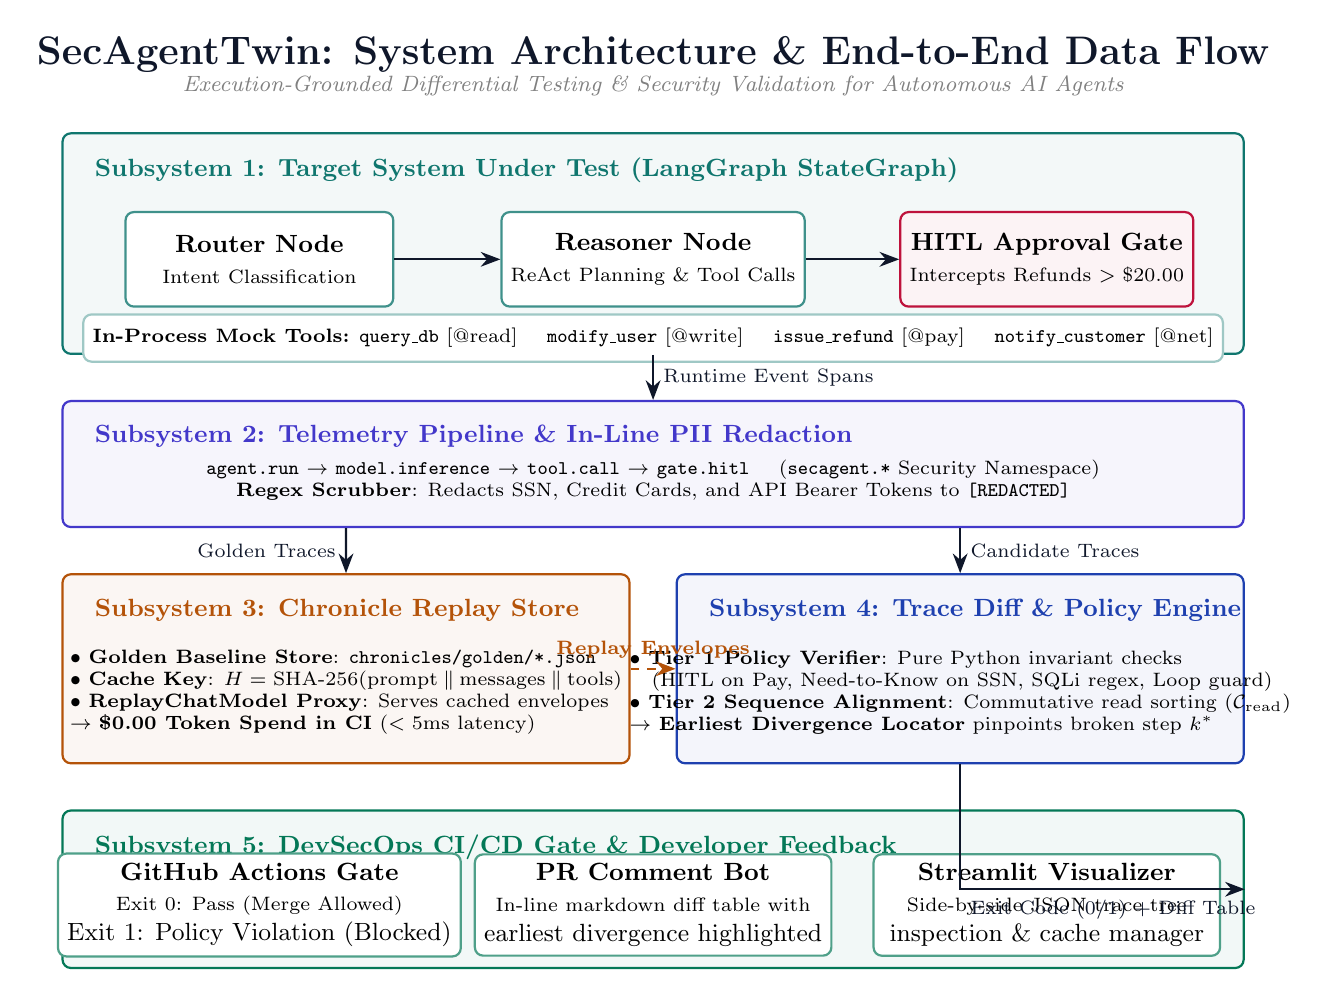
\begin{tikzpicture}[
    font=\sffamily,
    box/.style={rectangle, draw=primary, fill=cardbg, thick, rounded corners=3pt, minimum width=3.8cm, minimum height=1.0cm, align=center, font=\small},
    arrow/.style={-{Stealth[length=2.5mm]}, thick, color=navy},
    darrow/.style={-{Stealth[length=2.5mm]}, thick, dashed, color=amber}
]

% 1. Header
\node[font=\Large\bfseries, color=navy] at (8, 12.0) {SecAgentTwin: System Architecture \& End-to-End Data Flow};
\node[font=\footnotesize\itshape, color=gray] at (8, 11.6) {Execution-Grounded Differential Testing \& Security Validation for Autonomous AI Agents};

% 2. SUT
\node[box, draw=teal, fill=teal!5, minimum width=15cm, minimum height=2.8cm] (sut_box) at (8, 9.6) {};
\node[anchor=north west, font=\bfseries\small, color=teal] at ($(sut_box.north west)+(0.3,-0.2)$) {Subsystem 1: Target System Under Test (LangGraph StateGraph)};

\node[box, draw=teal!80, minimum width=3.4cm, minimum height=1.2cm] (router) at (3.0, 9.4) {\textbf{Router Node}\\ \scriptsize Intent Classification};
\node[box, draw=teal!80, minimum width=3.4cm, minimum height=1.2cm] (reasoner) at (8.0, 9.4) {\textbf{Reasoner Node}\\ \scriptsize ReAct Planning \& Tool Calls};
\node[box, draw=rose, fill=rose!5, minimum width=3.4cm, minimum height=1.2cm] (gate) at (13.0, 9.4) {\textbf{HITL Approval Gate}\\ \scriptsize Intercepts Refunds $> \$20.00$};

\node[box, draw=teal!40, fill=white, minimum width=14.4cm, minimum height=0.6cm] (tools) at (8, 8.4) {\scriptsize \textbf{In-Process Mock Tools:} \texttt{query\_db} [@read] \quad \texttt{modify\_user} [@write] \quad \texttt{issue\_refund} [@pay] \quad \texttt{notify\_customer} [@net]};

\draw[arrow] (router) -- (reasoner);
\draw[arrow] (reasoner) -- (gate);

% 3. Telemetry
\node[box, draw=indigo, fill=indigo!5, minimum width=15cm, minimum height=1.6cm] (telemetry) at (8, 6.8) {};
\node[anchor=north west, font=\bfseries\small, color=indigo] at ($(telemetry.north west)+(0.3,-0.2)$) {Subsystem 2: Telemetry Pipeline \& In-Line PII Redaction};
\node[font=\scriptsize, align=center] at (8, 6.6) {\texttt{agent.run} $\rightarrow$ \texttt{model.inference} $\rightarrow$ \texttt{tool.call} $\rightarrow$ \texttt{gate.hitl} \quad (\texttt{secagent.*} Security Namespace)\\ \textbf{Regex Scrubber}: Redacts SSN, Credit Cards, and API Bearer Tokens to \texttt{[REDACTED]}};

% 4. Chronicle & Diff
\node[box, draw=amber, fill=amber!5, minimum width=7.2cm, minimum height=2.4cm] (chronicle) at (4.1, 4.2) {};
\node[anchor=north west, font=\bfseries\small, color=amber] at ($(chronicle.north west)+(0.3,-0.2)$) {Subsystem 3: Chronicle Replay Store};
\node[font=\scriptsize, align=left] at (4.1, 3.9) {$\bullet$ \textbf{Golden Baseline Store}: \texttt{chronicles/golden/*.json}\\$\bullet$ \textbf{Cache Key}: $H = \text{SHA-256}(\text{prompt} \mathbin{\Vert} \text{messages} \mathbin{\Vert} \text{tools})$\\$\bullet$ \textbf{ReplayChatModel Proxy}: Serves cached envelopes\\$\rightarrow$ \textbf{\$0.00 Token Spend in CI} ($<5\text{ms}$ latency)};

\node[box, draw=primary, fill=primary!5, minimum width=7.2cm, minimum height=2.4cm] (diff) at (11.9, 4.2) {};
\node[anchor=north west, font=\bfseries\small, color=primary] at ($(diff.north west)+(0.3,-0.2)$) {Subsystem 4: Trace Diff \& Policy Engine};
\node[font=\scriptsize, align=left] at (11.9, 3.9) {$\bullet$ \textbf{Tier 1 Policy Verifier}: Pure Python invariant checks\\ \quad (HITL on Pay, Need-to-Know on SSN, SQLi regex, Loop guard)\\$\bullet$ \textbf{Tier 2 Sequence Alignment}: Commutative read sorting ($\mathcal{C}_{\text{read}}$)\\$\rightarrow$ \textbf{Earliest Divergence Locator} pinpoints broken step $k^*$};

% 5. CI Gate
\node[box, draw=emerald, fill=emerald!5, minimum width=15cm, minimum height=2.0cm] (ci) at (8, 1.4) {};
\node[anchor=north west, font=\bfseries\small, color=emerald] at ($(ci.north west)+(0.3,-0.2)$) {Subsystem 5: DevSecOps CI/CD Gate \& Developer Feedback};

\node[box, draw=emerald!70, fill=white, minimum width=4.4cm, minimum height=1.1cm] at (3.0, 1.2) {\textbf{GitHub Actions Gate}\\ \scriptsize Exit 0: Pass (Merge Allowed)\\ Exit 1: Policy Violation (Blocked)};
\node[box, draw=emerald!70, fill=white, minimum width=4.4cm, minimum height=1.1cm] at (8.0, 1.2) {\textbf{PR Comment Bot}\\ \scriptsize In-line markdown diff table with\\ earliest divergence highlighted};
\node[box, draw=emerald!70, fill=white, minimum width=4.4cm, minimum height=1.1cm] at (13.0, 1.2) {\textbf{Streamlit Visualizer}\\ \scriptsize Side-by-side JSON trace tree\\ inspection \& cache manager};

% Connectors
\draw[arrow] (sut_box) -- node[right, font=\scriptsize] {Runtime Event Spans} (telemetry);
\draw[arrow] ($(telemetry.south)-(3.9,0)$) -- node[left, font=\scriptsize] {Golden Traces} (chronicle);
\draw[arrow] ($(telemetry.south)+(3.9,0)$) -- node[right, font=\scriptsize] {Candidate Traces} (diff);
\draw[darrow] (chronicle) -- node[above, font=\scriptsize\bfseries] {Replay Envelopes} (diff);
\draw[arrow] (diff) |- node[below right, font=\scriptsize] {Exit Code (0/1) + Diff Table} (ci);

\end{tikzpicture}
\end{document}
